\documentclass{bioinfo}
\copyrightyear{2014}
\pubyear{2014}

\begin{document}
\firstpage{1}

\title[DNAplotlib]{DNAplotlib: standardized visualization of genetic constructs, libraries and associated data}
\author[Thomas E. Gorochowski \textit{et~al.}]{Thomas~E.~Gorochowski$^{1}$, Bryan~Der$^{1}$, Emerson~Glassey$^{1}$, D. Benjamin Gordon$^{1}$ and Christopher~A.~Voigt$^{1,}$\footnote{to whom correspondence should be addressed}}
\address{$^{1}$Department of Biological Engineering, Synthetic Biology Center, Massachusetts Institute of Technology, USA.}

\history{Received on XXXXX; revised on XXXXX; accepted on XXXXX}

\editor{Associate Editor: XXXXXXX}

\maketitle

\begin{abstract}

\section{Summary:}
DNAplotlib is a computational toolkit that enables highly customizable visualization of single genetic constructs and libraries of design variants. Publication quality vector-based output is produced and all aspects of the rendering process can be easily customized or extended by the user. DNAplotlib is capable of outputting SBOL Visual compliant diagrams, in addition to a trace-based format that is able to better illustrate the precise location and length of each genetic part. This alternative visualization method enables direct comparison with nucleotide-level data such as RNA-seq read depth. While it is envisaged that access will be predominantly via the programming interface, a web front-end is also provided to support broader usage.

\section{Availability:}
DNAplotlib is cross-platform and open-source software developed using Python and released under the OSI recognized NPOSL-3.0 licence. Source code, documentation and a web front-end are available at the project website: \href{http://www.dnaplotlib.org}{http://www.dnaplotlib.org}.

\section{Contact:} \href{cavoigt@gmail.com}{cavoigt@gmail.com}
\end{abstract}

% Background to standardized designs... highlight the problem
Engineering disciplines rely on standardized pictorial representations of parts and their interconnections to clearly communicate how these should be pieced together to form a design, and allow for the reliable construction of large complex systems. In biology, DNA sequences are often engineered to create genetic constructs that probe or perturb the function of natural systems, or more recently, create novel capabilities in what has been termed ``synthetic biology''. Unlike traditional engineering fields, the way that these designs are visually represented varies significantly between labs and sub-disciplines of the field, leading to ambiguities that can hinder understanding and the effective reuse of this research. The Synthetic Biology Open Language (SBOL) Visual initiative was started to help alleviate this problem by defining a set of agreed symbols for commonly used genetic elements \citep{Quinn13a}. However, so far this standard has seen limited uptake due to a lack of accessible tools that can be directly integrated into existing design and analysis workflows.

% Clearly explain what we have created and how it fills this void
To tackle this issue we developed DNAplotlib, a computational toolkit that facilitates the allows for the 

% Place in the context of existing literature/tools. Why don't these solve the problems highlighted
Some attempts to simplify the creation of standard-compliant diagrams have been made. The most prominent of these is PigeonCAD \citep{Bhatia13a}, a web-based tool that interprets a text-based syntax for specifying a genetic design and automatically transforms this into a visual representation. While this tool is Unfortunately, this tool is hampered by several limitations. The biggest limitation of these approaches so far though is an inability to integrate with existing scientific computing visualization and analysis tools. This is essential as 

% Libraries in synthetic biology and growing need to automate these processes.
% 2. (1 para). Existing tools that are available and the current difficulties in using them, e.g., PigeonCAD \citep{Bhatia13a}. Why is it needed... difficulty with library designs \citep{Smanski14a,Bilitchenko11a}.
Another growing area of research that is not well supported by such existing tools is the push towards automated design procedures that harness the potential to construct huge libraries of design variants \citep{Smanski14a,Bilitchenko11a}. Under these scenarios, automation of visualization tasks is essential to ensure clear communication of these large and diverse design spaces. No existing tools are available to support this need. 





As synthetic biology moves ever closer to automated design procedures that harness the potential to construct huge libraries of design variants \citep{Smanski14a,Bilitchenko11a}, supporting visualization tools will become important to ensure clear communication of these large and diverse designs. The SBOL Visual initiative was started to aid in this task with the definition of agreed pictorial representations of genetic elements \citep{Quinn13a}. However, so far it has seen limited uptake due to a lack a tools that are able to be easily integrated into existing analysis work-flows. DNAplotlib fills this gap by providing a computational toolkit that both adheres to this standard while also enabling highly customizable visualizations that are most appropriate for the specific needs of the laboratory. It is hoped that by providing researchers with this flexibility that they will be more willing to apply such standards to their work, improving general uptake of SBOL Visual across the field.

\begin{figure}[t]
\centering
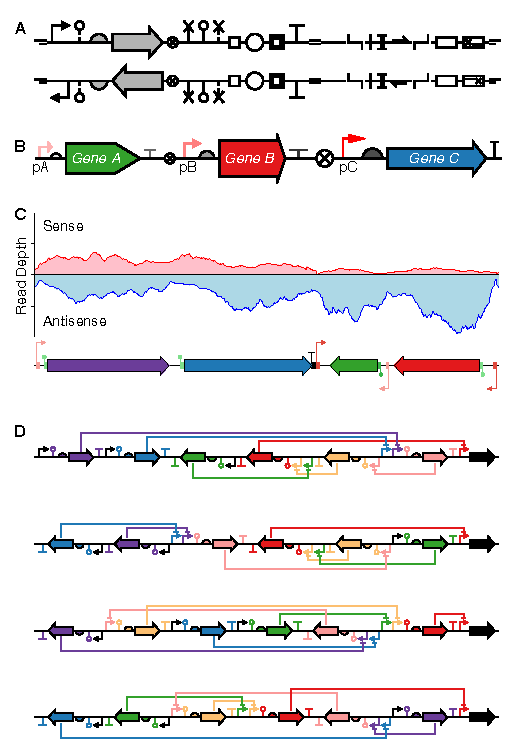
\includegraphics[width=8.3cm]{Figure1.pdf}
\caption{\label{fig:overview}Overview of core DNAplotlib functionality. (\textbf{A})~The complete set of SBOL Visual parts that capture the majority of widely used genetic elements is available for use in both forward and reverse orientations. (\textbf{B})~The size, color, shape and labeling of all elements can be easily customized allowing for additional information to be communicated e.g., promoter strengths or spacer lengths. Users can further supply their own functions to draw parts in a non-standard way or to represent new types of genetic element yet to be incorporated into SBOL Visual. (\textbf{C})~To allow for direct comparison between a genetic design and associated nucleotide-level data, such as RNA-seq read depths, trace-based renderers are also provided. These use the standard promoter and terminator symbols and a small filled circle to represent an RBS. Indicators of actual part widths (arrow length for CDSs and small filled rectangles for promoters and RBSs) are displayed on the DNA backbone to enable a clear visual alignment of design information with trace data. (\textbf{D})~Visualization of a library of genetic design variants implementing the same 3-input (black promoters), 1-output (black CDS) device. Colors have been used to link repressor genes to their cognate promoters.}
\end{figure}

% Technicalities of DNAplotlib
% 3. (3 para). What DNAplotlib is: Python-based, uses matplotlib \citep{Hunter07a}, generates publication quality vector-based output. Highly customizable at all stages of the rendering process. Enables both single and libraries to be easily visualized. Describe the rendering pipeline, and multiple types of output available.
To address these needs DNAplotlib has been built using matplotlib \citep{Hunter07a}, a highly portable Python-based 2D graphics library that allows for graphical output in the form of vector based PDFs or rasterized PNG or JPEG images. A major advantage oFurthermore, it enables the rendering of genetic designs to be easily integrated into existing analysis scripts. Python was chosen due to its increasing use for the analysis of biological data \citep{Cock09a} and its availability across all major operating systems.

% Rendering pipeline
A key consideration in the design of DNAplotlib was ensuring all aspects of the rendering process could be customized to specific user requirements. As fields such as synthetic biology are still evolving, the the precise way in which such tools will be used and the discovery of new types of genetic part that need to be included, but may not yet have a standardized representation. Enabling custom elements to be easily added and refined over time will ensure such elements are captured and also contribute to the standardization process. 

dictionary that contains core attributes corresponding to part type and orientation, in addition to other attributes that influence the style of the part. Attributes that are not used by a particular renderer are ignored, meaning that it is easy to swap these functions without fear of breaking the entire rendering pipeline.

% Scripts to ease use - text based input, simple construct definition language
To generate a 
In addition to direct library access through Python analysis scripts, we also provide two scripts to enable input in the form of text files

% Web-based interface. What does this include, what it doesn't. Why did we make it.
To ensure broadest application of these tools by non-programmers, a web-based interface was also developed. This allows for the visualization of single designs or the . Reduces the requirement of a user to have a working Python installation locally on their machine.
that allows text files describing part styles and DNA designs to be uploaded and processed. These files uploaded to the server, processed by the scripts described previously, and generated images are returned to the user. This ensures broadest use of the library and ensures that members across a lab can share the same styling of diagrams to ensure clear communication of their designs.

% Broader view. How is this toolkit going to help the community. Broader use of SBOL-compliant figures? Easier communication of ideas. Still able to have a lab ``style'' to differentiate your work and emphasize aspects in unique ways.
We see a key feature of ensuring adoption as 

% Future directions (general point on where it is available and potential for external contributions)
DNAplotlib is under continual development with a current focus on broadening the types of genetic element covered to include new synthetic biological parts. The project welcomes contributions from others within the community through the project website and public development repository: \href{http://www.dnaplotlib.org}{http://www.dnaplotlib.org}.

\section*{ACKNOWLEDGEMENTS}
T.E.G., B.D., E.G., D.B.G. and C.A.V. were supported by...

\begin{thebibliography}{}
	
\bibitem[Bhatia \& Densmore, 2013]{Bhatia13a} Bhatia, S. and Densmore, D. (2013). Pigeon: A Design Visualizer for Synthetic Biology, {\it ACS Synth. Biol.}, {\bf 2}, 348-350.

\bibitem[Smanski {\it et~al}., 2014]{Smanski14a} Smanski, M.J., Swapnil, B., Park, YJ., Zhao, D., Giannoukos, G., Ciulla, D., Busby, M., Calderon, J., Nicol, R., Gordon, D.B., Densmore, D. and Voigt, C.A. (2014) Combinatorial design and assembly of refactored gene clusters, {\it Nat. Biotech.}, {\bf ?}, ???-???.

\bibitem[Hunter, 2007]{Hunter07a} Hunter, J.D. (2007). Matplotlib: A 2D graphics environment, {\it Computing in Science \& Engineering}, {\bf 9}, 90-95.

\bibitem[Cock {\it et~al}., 2009]{Cock09a} 
Cock PJ, Antao T, Chang JT, Chapman BA, Cox CJ, Dalke A, Friedberg I, Hamelryck T, Kauff F, Wilczynski B, and de Hoon MJ. (2009) Biopython: freely available Python tools for computational molecular biology and bioinformatics. {\it Bioinformatics}, {\bf 25}, 1422-1422.

\bibitem[Bilitchenko {\it et~al}., 2011]{Bilitchenko11a} 
Bilitchenko, L., Liu, A., Cheung, S., Weeding, E., Xia, B., Leguia, M., Anderson, J.C., Densmore, D. (2011) Eugene – A Domain Specific Language for Specifying and Constraining Synthetic Biological Parts, Devices, and Systems. {\it PLoS ONE}, {\bf 6}, e18882.

\bibitem[Quinn {\it et~al}., 2013]{Quinn13a} 
Quinn, J., Beal, J., Bhatia, S., Cai, P., Chen, J., Clancy, K., Hillson, N., Galdzicki, M., Maheshwari, A.P., Umesh; P., Matthew; R.C.; Stan, G.-B., Endy, D. (2013) ``Synthetic Biology Open Language Visual (SBOL Visual), version 1.0.0.''

\end{thebibliography}

\end{document}



%The SBOL Visual initiative was started to aid in this task with the definition of agreed pictorial representations of genetic elements \citep{Quinn13a}. However, so far it has seen limited uptake due to a lack a tools that are able to be easily integrated into existing analysis work-flows. DNAplotlib fills this gap by providing a computational toolkit that both adheres to this standard while also enabling highly customizable visualizations that are most appropriate for the specific needs of the laboratory. It is hoped that by providing researchers with this flexibility that they will be more willing to apply such standards to their work, improving general uptake of SBOL Visual across the field.
